%/*******************************************************************************
% * Copyright (c) 2009, medshare GmbH
% * All rights reserved. This program may not be distributed
% * or modified without prior written consent
% *
% * Contributors:
% *    T. Schaller - initial implementation
% *
% *******************************************************************************/
\documentclass[a4paper]{scrartcl}
\usepackage{german}
\usepackage[utf8]{inputenc}
\usepackage{makeidx}
\usepackage{wrapfig}
\makeindex

\usepackage[pdftex]{graphicx}
\DeclareGraphicsExtensions{.pdf,.jpg,.png}

\usepackage{floatflt}
\usepackage[]{hyperref}
\usepackage{color}
\title{Elexis - Afinion AS100 Connector}
\author{medshare GmbH}

\begin{document}

%\extratitle{
%    \vfill
%	\begin{center}
%		
\includegraphics{elexis_logo}
%	\end{center}
%	\begin{center}
%		
\includegraphics{elexis_logo}
%	\end{center}
%    \begin{center}
%    Handbuch für die Abrechnung nach Tarmed
%    \end{center}
%    \vfill
%    \begin{center}
%   \copyright 2009 by medshare GmbH. Nachdruck und Weitergabe, auch auszugsweise, sowohl in elektronischer als auch in Papierform, nur mit Genehmigung des Autors oder von Axis-Shield.
%
%    \end{center}
%    \vfill
%}
\maketitle
	\begin{center}
		
\includegraphics{elexis_logo}
	\end{center}
	\begin{center}
		
\includegraphics{axis-shield_logo}
	\end{center}
	\begin{center}
		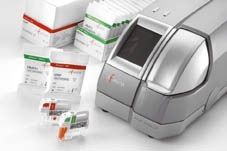
\includegraphics{afinion_device}
	\end{center}
	\begin{center}
		
\includegraphics{afinion_logo}
	\end{center}
\pagebreak

\section{Einführung}
TODO\\
Dieses Plugin dient dazu, das Laborgerät 'Afinion AS100 Analyzer'\footnote{Firma Axis-Schield} an Elexis anzubinden. Mit diesem Plugin können die vom Analyzer gemessenen Laborparameter direkt in die Elexis-Datenbank eingelesen werden.

\subsection{Voraussetzungen}
Dieses Plugin benötigt Elexis 1.4.0 oder höher sowie einen Afinion AS100 Analyzer. Ausserdem wird ein PC mit mindestens einer freien seriellen Schnittstelle und ein korrekt gerade verdrahtetes serielles Kabel (kein Nullmodemkabel) zur Verbindung des Analyzers mit dem PC benötigt.

\section{Installation und Konfiguration}
Installieren Sie auf dem im Labor befindlichen PC das Plugin wie gewohnt. Verbinden Sie dann bei \textbf{ausgeschalteten} Ger\u00E4ten den Analyzer mit der einem seriellen Port des Computers. Die serielle Datenkommunikation kann am Analyzer nicht eingestellt werden und ist standardm\u00E4ssig aktiv.

Starten Sie dann Elexis und gehen Sie dort zu \textsc{Datei-Einstellungen-Datenaustausch-Afinion AS100 Analyzer} (S. Abb. \ref{fig:config}).
%\begin{figure}[h]
%    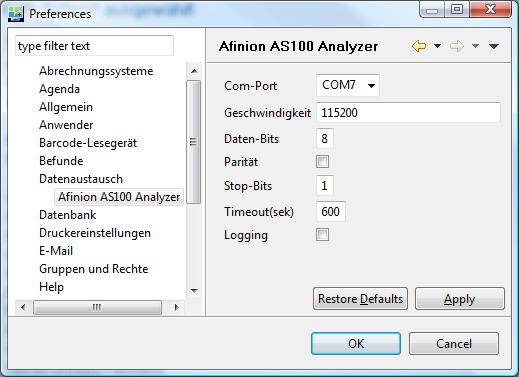
\includegraphics{config}
%    \caption{Einstellungen Afinion AS100 Analyzer}
%    \label{fig:config}
%\end{figure}
%Hier stellen Sie den seriellen Port und die Schnittstellenparameter ein.
%
%
%\section{Verwendung}
%\begin{figure}[h]
%    
\includegraphics{toolbarbutton}
%    \caption{Afinion AS100 Analyzer Daten einlesen}
%    \label{fig:toolbarbutton}
%\end{figure}
Wenn das Plugin korrekt installiert ist, erscheint in der Labor-View automatisch ein neuer Toolbar Button 'Afinion AS100 Analyzer' (Abb. \ref{fig:toolbarbutton}. Klicken Sie auf diesem Knopfum die Verbindung mit dem Ger\u00E4t herzustellen. Die Verbindung bleibt bestehen (Der Knopf erscheint eingerastet), bis entweder die Daten empfangen worden sind, oder TODO Minuten verstrichen sind, ohne dass Daten übertragen wurden, oder Sie den Knopf wieder manuell auslösen.

Dieses Plugin wurde unter Windows XP und Vista getestet. Beachten Sie bitte, dass unter Linux die seriellen Ports nicht COM1 usw., sondern /dev/ttyS0 usw. heissen.

\end{document}
